\documentclass{article}

\usepackage{graphicx}

\title{Report 3: Convert Color to GrayScale Image by Cuda}
\author{Le Nhu Chu Hiep}

\begin{document}
\maketitle

\begin{itemize}
    \item First thing: define grayScale function following slide example.
    \item Malloc space for cuda dev input and dev output
    \item Mem copy input buffer to dev input
    \item run grayScale function
    \item copy dev output to output
    \item free cuda malloc
\end{itemize}

Result in console:
\begin{verbatim}
USTH ICT Master 2018, Advanced Programming for HPC.
Warming up...
Starting labwork 3
labwork 3 ellapsed 144.3ms
\end{verbatim}

Result Image:
\begin{figure}
        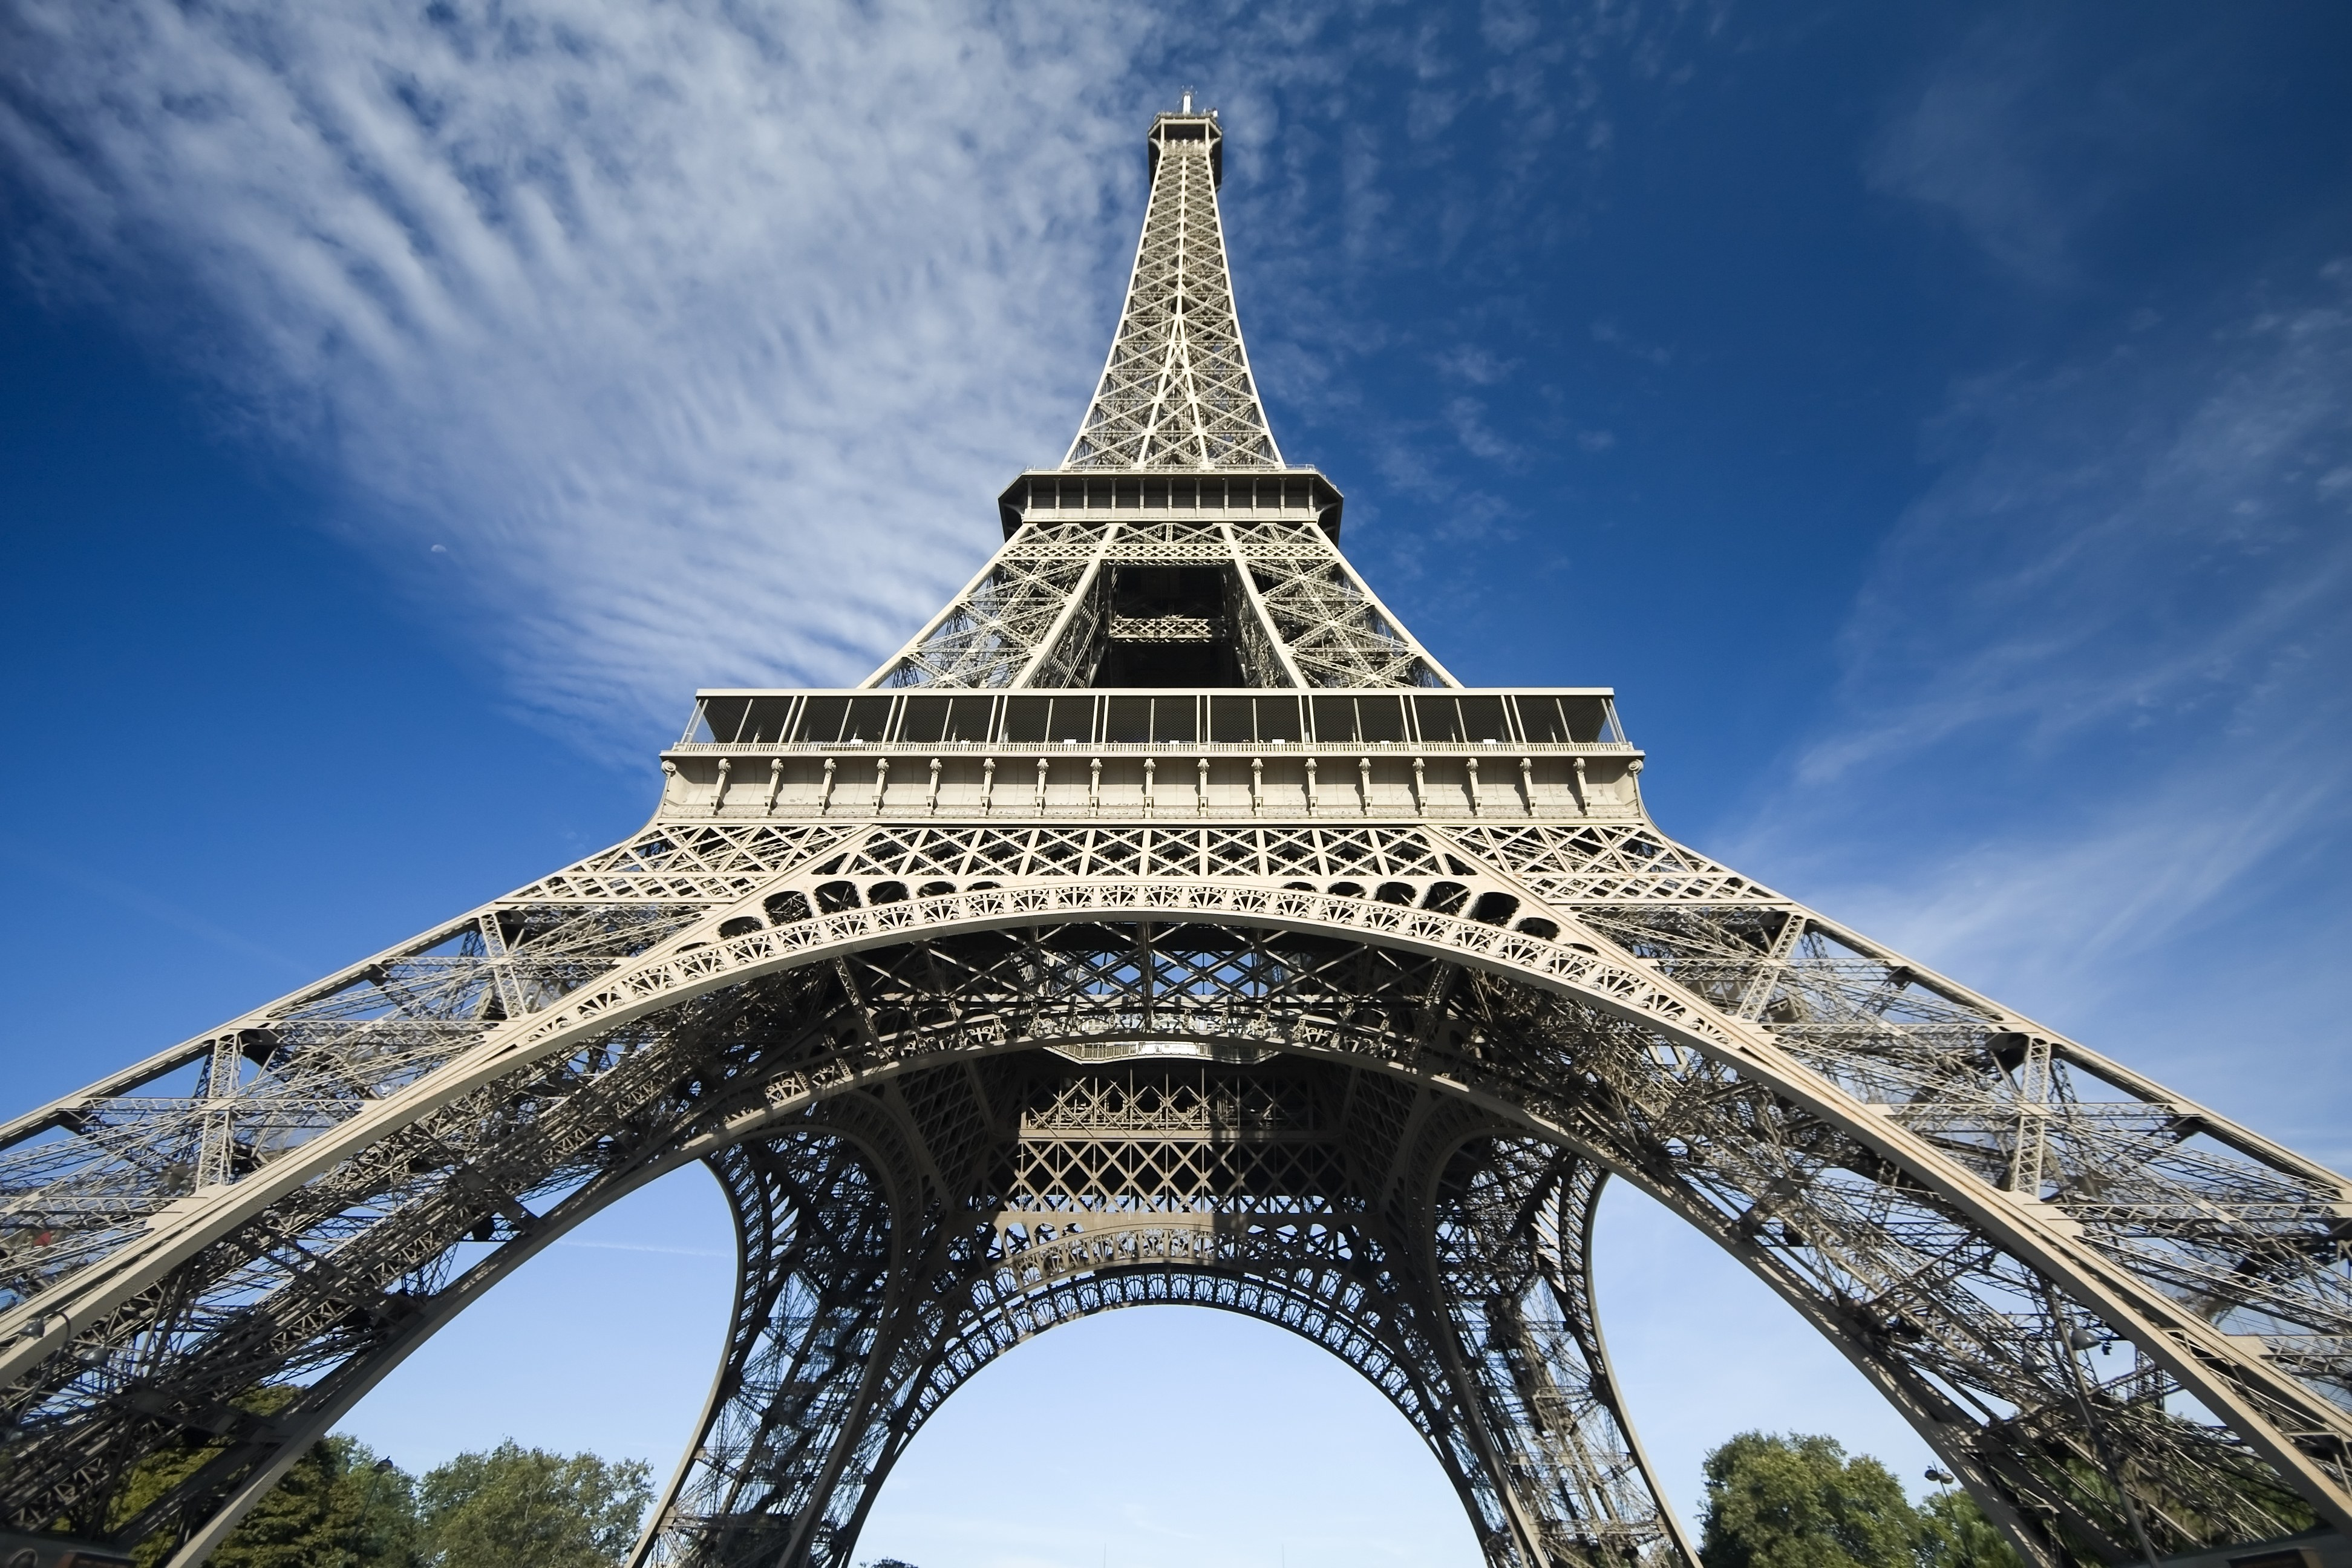
\includegraphics[width=\textwidth]{./labwork/data/eiffel.jpg}
        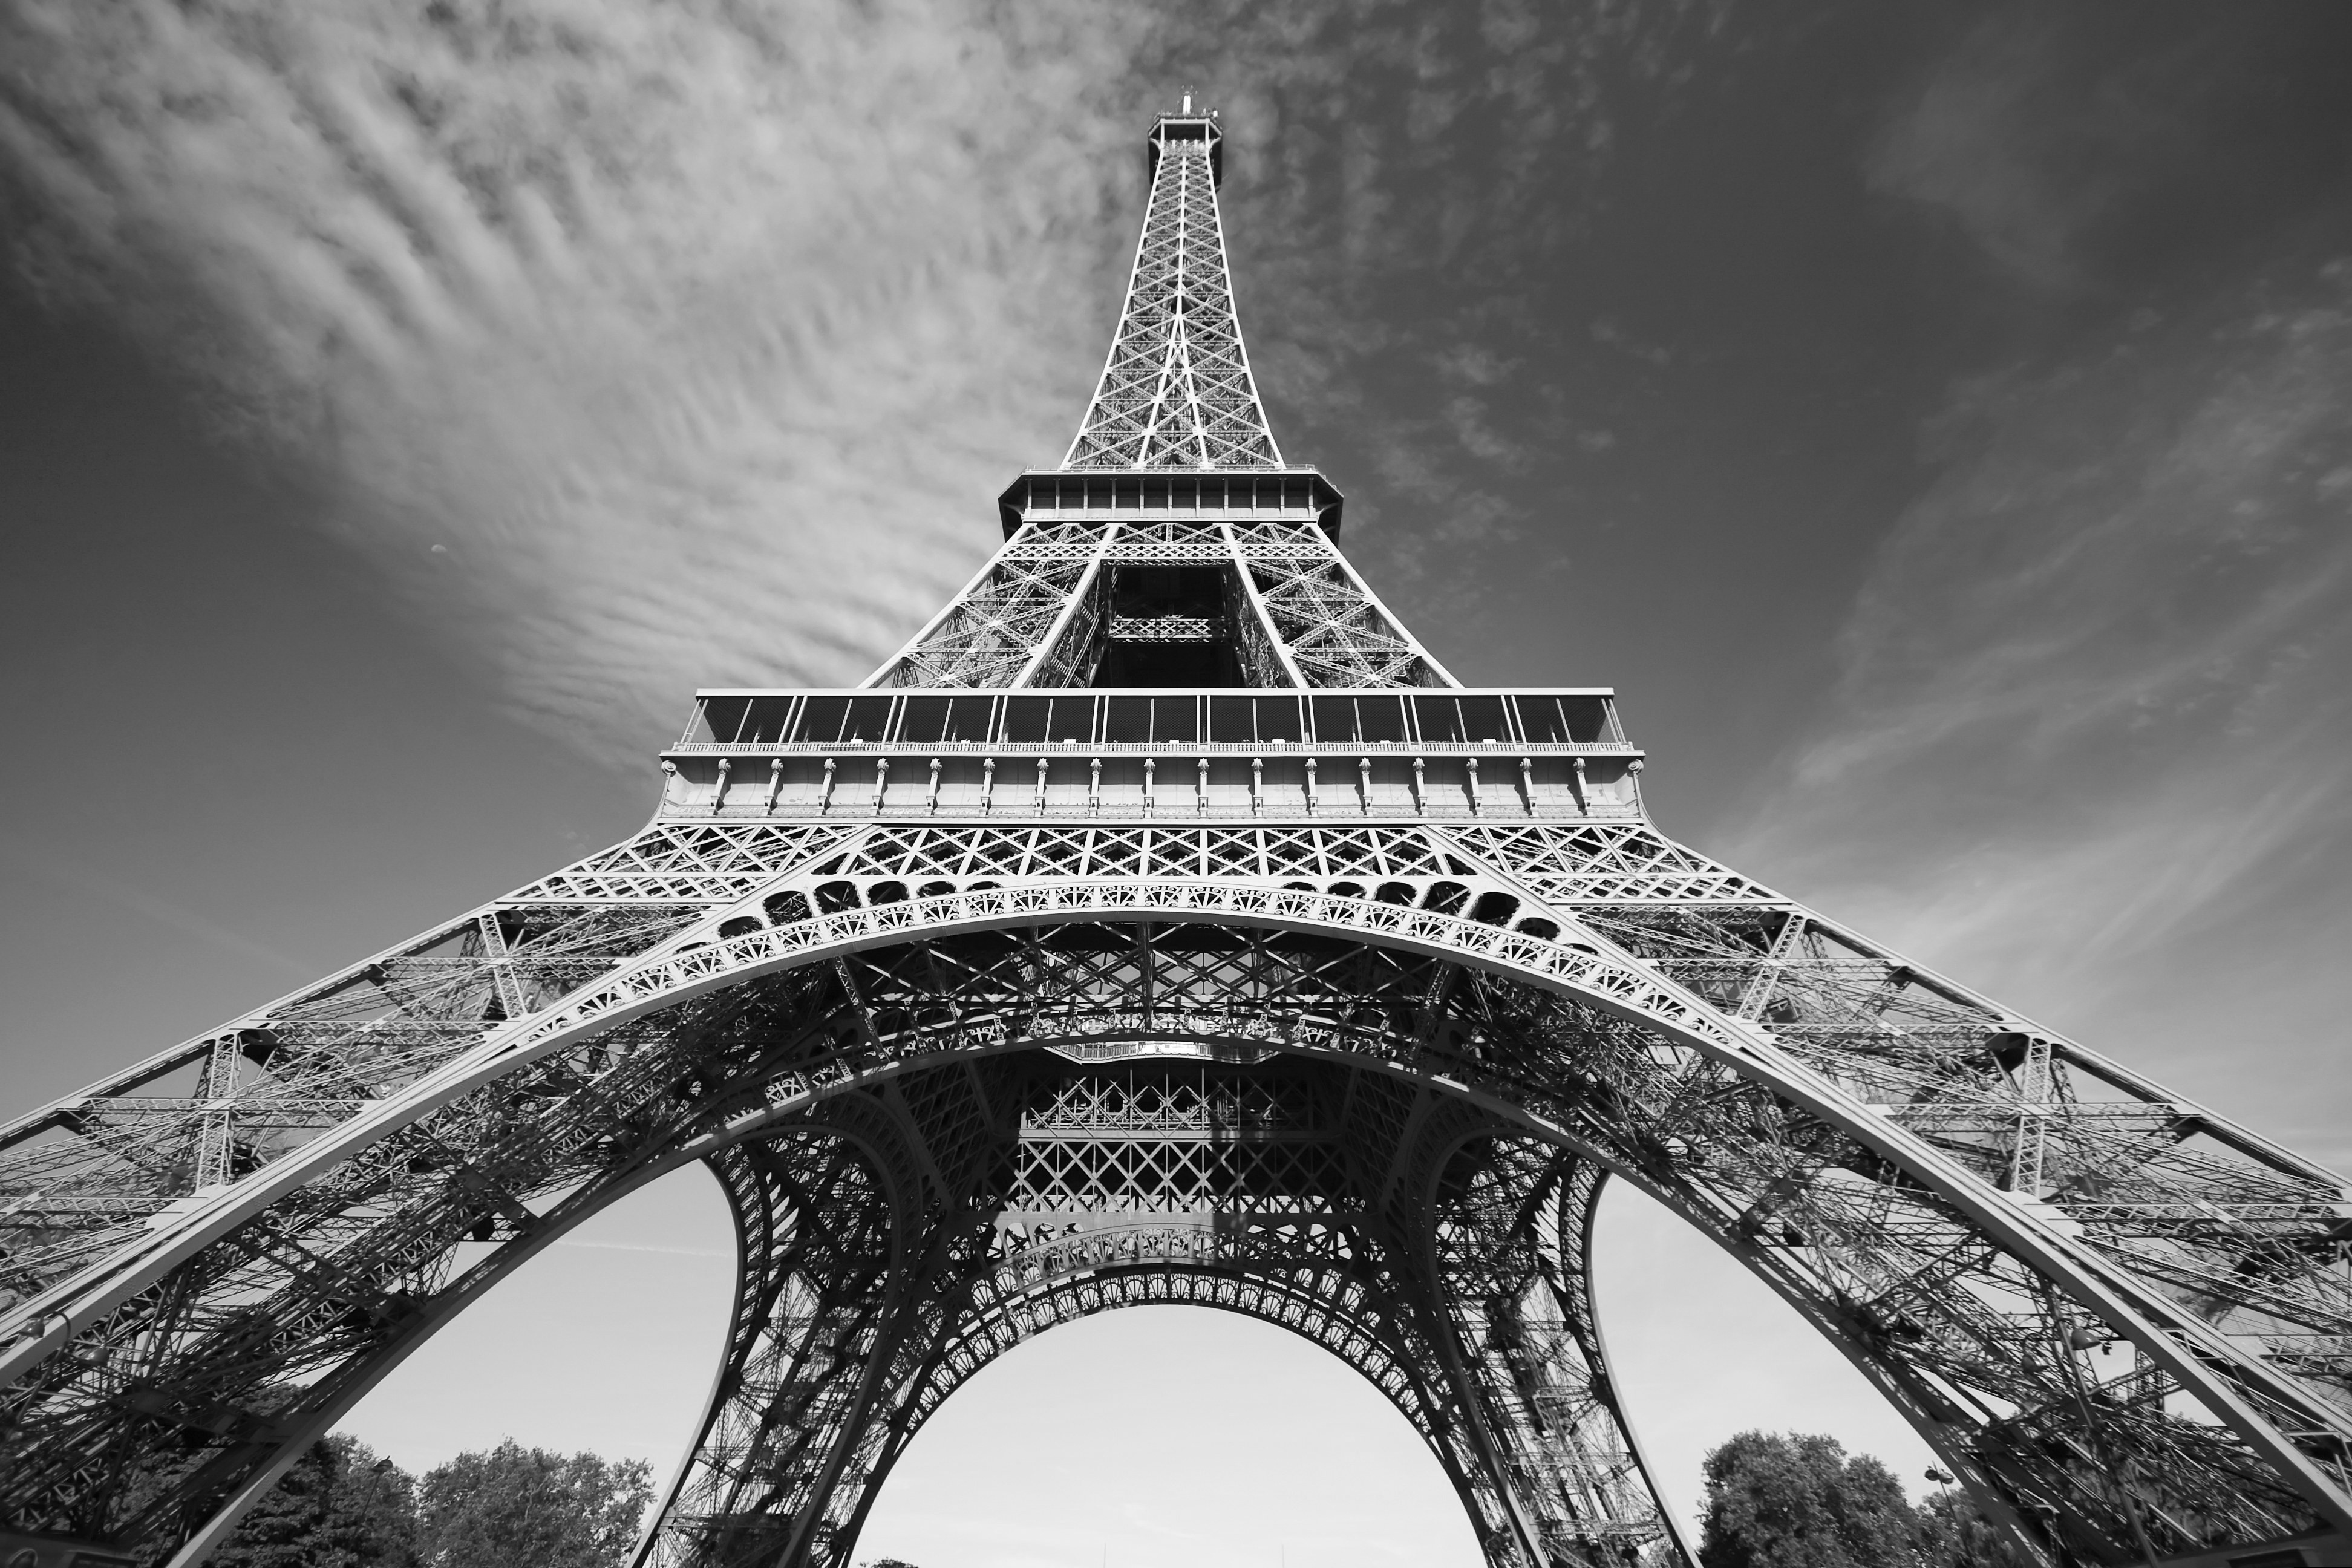
\includegraphics[width=\textwidth]{./labwork3-gpu-out.jpg}
        \caption{Eiffel Image}
\end{figure}
\end{document}
